\documentclass[a4paper,14pt,russian]{extreport}

%Чтобы работали все шрифты
\usepackage{extsizes}
%\usepackage{cmap} % для кодировки шрифтов в pdf
\usepackage[T2A]{fontenc}
\usepackage[utf8]{inputenc}
\usepackage[russian]{babel}


%Для рисуночков
%\usepackage[pdftex]{graphicx}
%\graphicspath{{figures/}}
%\DeclareGraphicsExtensions{.pdf,.png,.jpg}
\usepackage[pdftex]{graphicx}
\usepackage{float}
\graphicspath{{figures/}}
\DeclareGraphicsExtensions{.pdf,.png,.jpg}
\usepackage{indentfirst}
\usepackage[left=2cm,right=2cm,
    top=2cm,bottom=2cm,bindingoffset=0cm]{geometry}


\usepackage{amssymb,amsfonts,amsmath,amsthm}
\usepackage{indentfirst}
\usepackage[usenames,dvipsnames]{color}
\usepackage{makecell}
\usepackage{multirow}

%Настройка заголовков
\usepackage{titlesec}
 \titleformat{\chapter}[display]
    {\filcenter}
    {\MakeUppercase{\chaptertitlename} \thechapter}
    {8pt}
    {\bfseries}{}
 \titleformat{\section}
    {\normalsize\bfseries}
    {\thesection}
    {1em}{}
 \titleformat{\subsection}
    {\normalsize\bfseries}
    {\thesubsection}
    {1em}{}
    
 % Настройка вертикальных и горизонтальных отступов
\titlespacing*{\chapter}{0pt}{-30pt}{8pt}
\titlespacing*{\section}{\parindent}{*4}{*4}
\titlespacing*{\subsection}{\parindent}{*4}{*4}


 
\linespread{1.3}
\renewcommand{\rmdefault}{ftm}
\frenchspacing


\usepackage{tocloft}
\renewcommand{\cfttoctitlefont}{\hspace{0.38\textwidth} \bfseries\MakeUppercase}
\renewcommand{\cftbeforetoctitleskip}{-1em}
\renewcommand{\cftaftertoctitle}{\mbox{}\hfill \\ \mbox{}\hfill{\footnotesize Стр.}\vspace{-2.5em}}
\renewcommand{\cftchapfont}{\normalsize\bfseries \MakeUppercase{\chaptername} }
\renewcommand{\cftsecfont}{\hspace{31pt}}
\renewcommand{\cftsubsecfont}{\hspace{11pt}}
\renewcommand{\cftbeforechapskip}{1em}
\renewcommand{\cftparskip}{-1mm}
\renewcommand{\cftdotsep}{1}
\setcounter{tocdepth}{2} % задать глубину оглавления — до subsection включительно

\usepackage[tableposition=top]{caption}
\usepackage{subcaption}
\DeclareCaptionLabelFormat{gostfigure}{Рисунок #2}
\DeclareCaptionLabelFormat{gosttable}{Таблица #2}
\DeclareCaptionLabelSeparator{gost}{~---~}
\captionsetup{labelsep=gost}
\captionsetup[figure]{labelformat=gostfigure}
\captionsetup[table]{labelformat=gosttable}
\renewcommand{\thesubfigure}{\asbuk{subfigure}}


\usepackage{geometry}
\geometry{left=2.5cm}
\geometry{right=1cm}
\geometry{top=2cm}
\geometry{bottom=2cm}

\newcommand{\empline}{\mbox{}\newline}
\newcommand{\likechapterheading}[1]{ 
    \begin{center}
    \textbf{\MakeUppercase{#1}}
    \end{center}
    \empline}

\makeatletter
    \renewcommand{\@dotsep}{2}
    \newcommand{\l@likechapter}[2]{{\bfseries\@dottedtocline{0}{0pt}{0pt}{#1}{#2}}}
\makeatother
\newcommand{\likechapter}[1]{    
    \likechapterheading{#1}    
    \addcontentsline{toc}{likechapter}{\MakeUppercase{#1}}}


% Для работы с библиографией
\usepackage[square,numbers,sort&compress]{natbib}
\renewcommand{\bibnumfmt}[1]{#1.\hfill} % нумерация источников в самом списке — через точку
\renewcommand{\bibsection}{\likechapter{Список использованных источников}} % заголовок специального раздела
\setlength{\bibsep}{0pt}


\usepackage{fancyhdr} % пакет для установки колонтитулов
\pagestyle{fancy} % смена стиля оформления страниц
\fancyhf{} % очистка текущих значений
\fancyhead[C]{\thepage} % установка верхнего колонтитула
\renewcommand{\headrulewidth}{0pt} % убрать разделительную линию


\title{Бакалавр}
\author{Елисеев}
\date{The date}
\begin{document}
	\def\contentsname{СОДЕРЖАНИЕ}
	\begin{titlepage}
		\begin{center}
			\large Университет ИТМО\\[2cm]
			\huge Мой прекрасный диплом\\
			\large <<СВЕРХБЫСТРАЯ ДИНАМИКА НОСИТЕЛЕЙ ЗАРЯДА В ПОЛУПРОВОДНИКОВЫХ НИТЕВИДНЫХ НАНОКРИСТАЛЛАХ.>>\\[3cm]
			\begin{flushleft}
				\emph{Студент:} Елисеев А.\\
				\emph{Группа:} V3400\\
				\emph{Научрук:} Валерий Николаевич\\
			\end{flushleft}
			\vfill
			\large Санкт-Петербург\\
			\large 2017
		\end{center}
		\thispagestyle{empty} % без ном. стр.
	\end{titlepage}
	\setcounter{page}{2}
	\likechapter{Аннотация}
		\newpage
	\tableofcontents
	\chapter{Введение}
		\section{Актуальность темы работы.}
		Полупроводниковые наноструктуры в виде свободно стоящих
полупроводниковых нитевидных нанокристаллов (ННК), а так же отдельные ННК, являются одними из наиболее перспективных объектов для применения в наноэлектронике,
нанофотонике, а так же во многих других областях науки и техники. Так ННК используются для создания
сверхчувствительных фотодиодов \cite{semicondNNW2006}, транзисторов сверхвысокой плотности \cite{NNWtransistors}, эмиттеров излучения видимого диапазона волн \cite{singleNNWlaser} и ТГц диапазона \cite{THzGeneration}.\par
Огромная перспективность таких нанообъектов и структур на их основе обусловлена рядом уникальных электрических и оптических свойств. При создании метаповерхностей на основе свободно стоящих ННК, характерные размеры которых порядка $100 \text{ нм}$ в диаметре и $1 \text{ мкм}$ по высоте, получаются структуры с огромным по сравнению с объемными материалами соотношением площади поверхности к объему. В работе \cite{THzGeneration} было показано, что генерация ТГц излучения от упорядоченного массива ННК на основе $GaAs$ может быть практически в два раза эффективнее, чем от $InAs$ - объемного полупроводникового материала, который обладает наибольшей эффективностью генерации ТГц излучения. Такая высокая эффективность обусловлена именно тем, что соотношение площади поверхности к объему у таких структур значительно выше, чем у объемных материалов.\par
 При создании структур описанных в предыдущем параграфе, первостепенную важность занимает изучение вопроса влияния формы материала и ее размеров на динамику носителей заряда. Например, при значительном увеличении отношения площади поверхности к объему увеличивается вклад поверхностной рекомбинации носителей в материале. Таким образом время жизни электронов и дырок в наноструктурах на основе свободно стоящих полупроводниковых ННК может существенно отличаться от времени жизни в соответствующем объемном полупроводнике. Исследование этих отличий является основной задачей, которую необходимо решить перед тем, как использовать подобные материалы в качестве основы для базовых элементов наноэлектроники и нанофотоники.\par
Кроме того необходимо учитывать, что в полупроводниковых ННК при диаметрах порядка десятка нанометров и меньше и при концентрации $\geqslant 10^{17}\text{см}^{-3}$ процессы переноса в статических внешних полях описываются только продольной составляющей квазиимпульса, как это имеет место в
чисто одномерном ($1D$) случае. Динамика носителей заряда в таких структурах существенно отличается от динамики в объемных материалах. Например, в таких низкоразмерных системах как тонкие ННК, экранирование внешнего электромагнитного поля носит качественно иной характер, чем в объемных полупроводниках. Заряды, которые экранируют внешнее электромагнитное поле во всем пространстве, сами ограничены в своем движении одной линией. В связи с этим, эффективность экранирования в одномерных и квазиодномерных ННК значительно ниже, чем в случае трехмерных систем. Кроме того, как показано в \cite{SiliconNWContactPhenomena}, в одномерных структурах процессы релаксации происходят по диффузионному закону, а дрейф носителей вносит лишь небольшую поправку в эффективный коэффициент диффузии. В то же время в трехмерном случае релаксация заряда в основном определяется дрейфовыми процессами.\par

		\section{Транспорт, генерация и рекомбинация носителей в ННК.}
			В связи с высокой значимостью изучения временных характеристик носителей заряда и их транспорта в полупроводниковых ННК для различных областей науки и техники, на текущий момент представлено немало работ посвященных этой тематике.
			\subsection{Время жизни и подвижность носителей заряда.}
				На сегодняшний день многие научные группы изучают электрооптические свойства ННК на основе различных материалов. Так, значительный вклад в изучение влияния структуры полупроводниковых ННК на время жизни фототока и подвижность носителей в них сделали авторы \cite{CurrentLifetime}. В своей работе \cite{CurrentLifetime} авторы пользуясь методом  Optical-pump terahertz-probe spectroscopy, показали что покрытие ННК на основе $GaAs$ шубой $AlGaAs$ (материалом с более широкой запрещенной зоной) уменьшает плотность поверхностных ловушек до $82 \%$ тем самым увеличивая проводимость. Кроме того, им удалось установить, что двухтемпературный режим роста ННК на основе $GaAs$ почти удваивает подвижность носителей в ННК и втрое увеличивает время жизни свободных носителей.\par
				В их работе исследованы образцы четырех типов, СЭМ фотография образцов и схематичное изображение которых приведены на Рис. \ref{ris:NNWfromArticle}
				\begin{figure}[H]
					\center{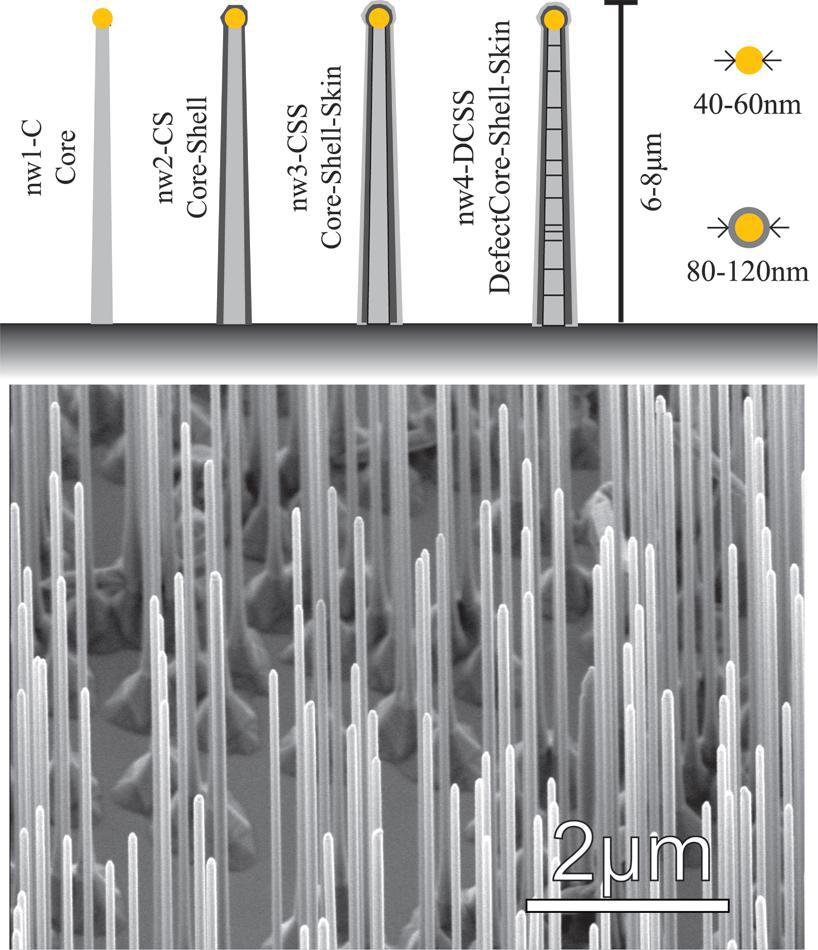
\includegraphics[width=0.6\linewidth]{NNWfromArticle}}
					\caption{СЭМ фотография образцов и их схематичное изображение. Рисунок взят из статьи \cite{CurrentLifetime}}
					\label{ris:NNWfromArticle}
				\end{figure}
				Авторы исследовали четыре вида ННК. Первые три вида были выращены при двухтемпературном режиме: nw1-C - обычные ННК на основе $GaAs$, nw2-CS - ННК на основе $GaAs$ с шубой $AlGaAs$ толщиной $\sim$ 30 нм, а на образце nw3-CSS поверх шубы $AlGaAs$ был еще нанесен тонкий слой $GaAs$ примерно 5 нм. Четвертых образец nw4-DCSS по структуре такой же как nw3-CSS, но выращен при однотемпературном режиме и поэтому подвержен двойному дефекту плотности.
			\subsection{Время релаксации электронов по импульсу.}
			\subsection{Особенности процессов диффузии и дрейфа носителей заряда.}

		\section{Генерация ТГц от массива полупроводниковых ННК}
			Коротко, о том, от чего зависит ТГц излучение от ННК. Определяющие процессы.
			
	\chapter{Основная часть}
			Далее речь пойдет о данной работе. Первое о чем будет рассказано - схема установки и описание экспериментального метода изучения динамики носителей в ННК. Динамикой в общем случае будем называть $\ldots$
			\newpage
		\section{Схема установки, описание метода}
			Ссылочка На статью, где впервые описан этот метод и его описание\par	
			Схема, ссылка на приложение, в котором описаны характеристики элементов, используемых в схеме.\par
			\newpage
		\section{Исследование ННК на основе $GaAs$}
			\subsection{Описание образцов и метода их получения}
				Метод газофазной эпитаксии, ссылка на
				статью и короткое описание\par
				Ориентация $GaAs$, получившиеся образцы,
				фото СЭМ
			\newpage
			\subsection{Зависимость эффективности генерации ТГц излучения от времени при возбуждении плазмы в образцах.}
				Типичный вид динамики\par
				Динамика, для упорядоченных образцов,
				при разной мощности накачки\par
				Характерные участки (короткая и длинная
				динамика)\par
			\subsection{Спад эффективности - экранировка встроенного поля}
			\subsection{Восстановление эффективности}
		\section{Исследование ННК на основе $GaAs/AlGaAs$}
			\subsection{Описание образцов и метода их получения}
				Метод газофазной эпитаксии, ссылка на
				статью и короткое описание\par
				Ориентация $GaAs$, получившиеся образцы,
				фото СЭМ
			\newpage
			\subsection{Зонные диаграммы ННК $GaAs$ и $GaAs/AlGaAs$}
			\subsection{Зависимость эффективности генерации ТГц излучения от времени при возбуждении плазмы в образцах.}
				Типичный вид динамики\par
				Динамика, для упорядоченных образцов,
				при разной мощности накачки\par
				Характерные участки (короткая и длинная
				динамика)\par
			\subsection{Спад эффективности.}
			\subsection{Восстановление эффективности.}
		\section{Исследование неупорядоченных массивов ННК на основе $GaAs$}
			\subsection{Описание образцов и метода их получения}
				Метод газофазной эпитаксии, ссылка на
				статью и короткое описание\par
				Ориентация $GaAs$, получившиеся образцы,
				фото СЭМ
			\newpage
			\subsection{Зависимость эффективности генерации ТГц излучения от времени при возбуждении плазмы в образцах.}
				Типичный вид динамики\par
				Динамика, для упорядоченных образцов,
				при разной мощности накачки\par
				Характерные участки (короткая и длинная
				динамика)\par
			\subsection{Спад эффективности - экранировка встроенного поля}
			\subsection{Восстановление эффективности}
		\section{Сравнение и анализ динамики носителей в разных образцах}
			Объяснение разницы в динамике
			\newpage
	\chapter{Заключение}
		\section{Положения дипломной работы}
			Все что удалось узнать, но в виде выражений и емких утверждений.
			\newpage
	\likechapter{Список сокращений и условных обозначений}
		\newpage
	\likechapter{Список терминов}
		\newpage
	\begin{thebibliography}{9}
		\bibitem{semicondNNW2006} Agarwal R., Lieber C. M. Semiconductor nanowires: optics and optoelectronics //Applied Physics A. – 2006. – Т. 85. – №. 3. – С. 209.
		\bibitem{NNWtransistors} Tomioka K., Yoshimura M., Fukui T. A III-V nanowire channel on silicon for high-performance vertical transistors //Nature. – 2012. – Т. 488. – №. 7410. – С. 189-192.
		\bibitem{singleNNWlaser} Duan X. et al. Single-nanowire electrically driven lasers //Nature. – 2003. – Т. 421. – №. 6920. – С. 241-245.
		\bibitem{THzGeneration} Trukhin V. N. et al. Generation of terahertz radiation in ordered arrays of GaAs nanowires //Applied Physics Letters. – 2015. – Т. 106. – №. 25. – С. 252104.
		\bibitem{SiliconNWContactPhenomena} Аверкиев Н.С., Шик А.Я.  Контактные явления в квантовых нитях и пористом кремнии//Физика и техника полупроводников. - 1996. - №.2 - С. 199
		\bibitem{CurrentLifetime} Parkinson P. et al. Carrier lifetime and mobility enhancement in nearly defectfree coreshell nanowires measured using time-resolved terahertz spectroscopy //Nano letters. – 2009. – Т. 9. – №. 9. – С. 3349-3353.
	\end{thebibliography}		
	\newpage 
	\likechapter{Приложения}
\end{document}



















